\paragraph{Scopo}

\paragraph{Sviluppo}
Lo sviluppo di \textit{G\&B} avviene seguendo il modello incrementale, spiegato nel dettaglio nel documento \textit{Piano di Progetto} alla sezione §4.\\
La proponente nel capitolato d'appalto pone un singolo vincolo riguardo le tecnologie da utilizzare:
\begin{itemize}
	\item JavaScript: in particolare nella sua declinazione nota come ECMAScript 6\glossario.
\end{itemize}
Tuttavia, ai fini della realizzazione del prodotto finale, il team \texttt{Agents of S.W.E.} ha definito l'uso di ulteriori tecnologie, analizzate brevemente di seguito, per scopi diversi:
\begin{itemize} 
	\item Telegraf\glossario\footnote{\url{https://www.influxdata.com/time-series-platform/telegraf/}}: è un agente per la raccolta e la rilevazione periodica di metriche\footnote{Metriche d'uso di un elaboratore. Per esempio: percentuale d'uso della CPU, pressione di memoria, etc.} e dati. Si connette ad un database\glossario e salva tali dati;
	\item InfluxDB\glossario\footnote{\url{https://www.influxdata.com/time-series-platform/influxdb/}}: è un database\glossario per le serie temporali. Verrà utilizzato per il salvataggio dei dati raccolti da Telegraf;
	\item jsbayes\glossario: libreria suggerita dal proponente per la semplice definizione di reti bayesiane; 
	\item UnBBayes\glossario\footnote{\url{https://sourceforge.net/projects/unbbayes/}}: framework e interfaccia grafica per le reti bayesiane. In particolare, verrà utilizzato per la visualizzazione della rete bayesiana in uso all'interno del plug-in, per soddisfare il requisito opzionale 2 esposto all'interno del capitolato d'appalto.
\end{itemize}

\begin{figure}[H]
	\begin{center}
		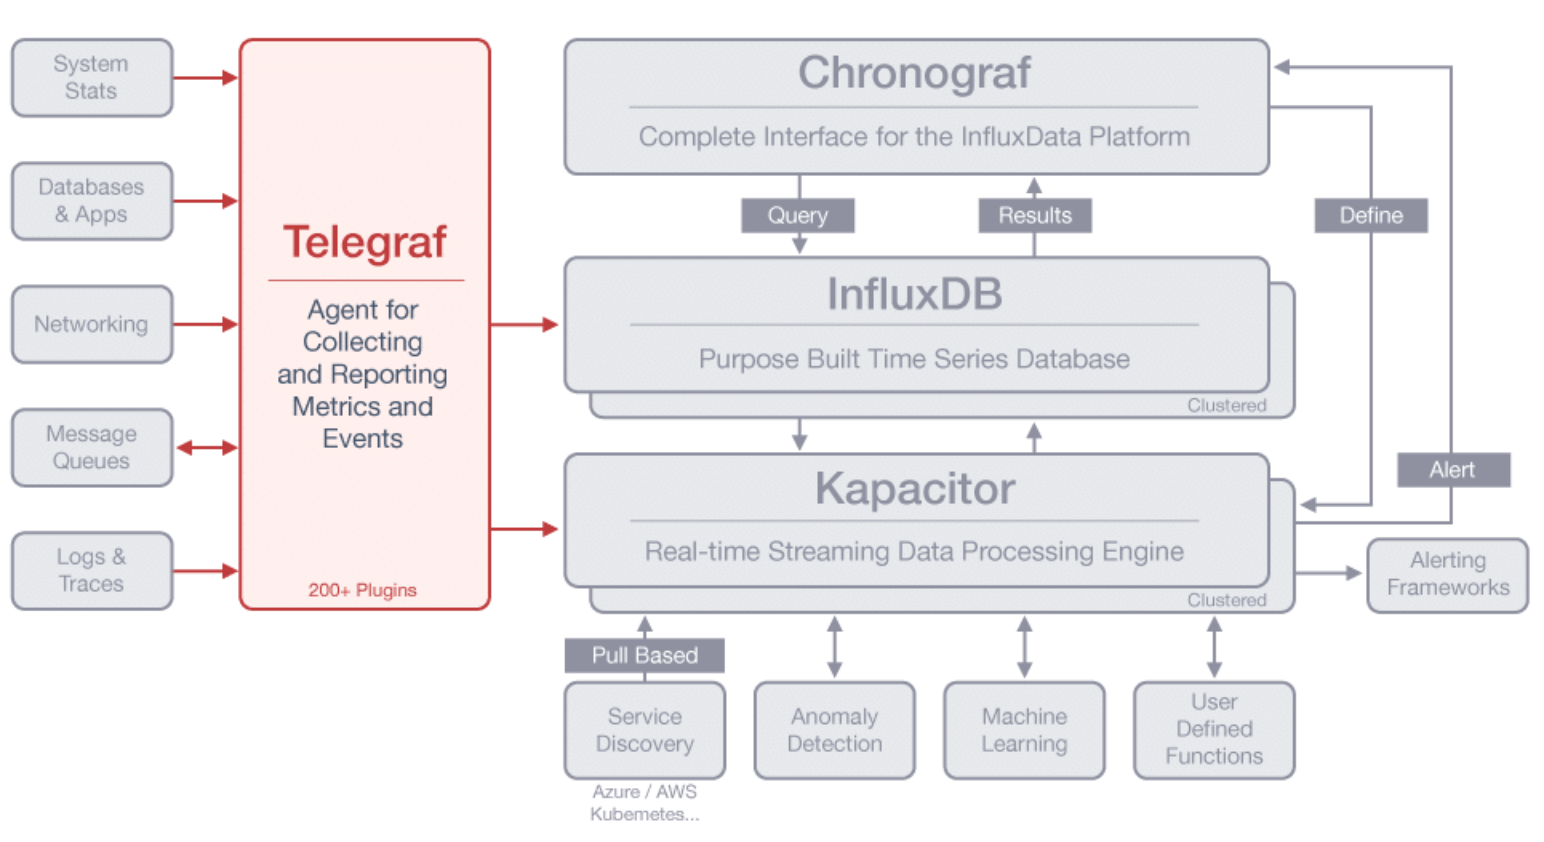
\includegraphics[scale=0.25]{./images/influxTelegraf.jpg}
		\caption{Rappresentazione del funzionamento di Telegraf e InfluxDB. Immagine dal sito web del produttore: \url{https://www.influxdata.com/time-series-platform/telegraf}}
	\end{center}
\end{figure}



\paragraph{Integrazione}

\paragraph{Diagrammi}

\paragraph{Obiettivi della progettazione}